\documentclass[hidelinks,12pt]{article}
\usepackage[left=0.25cm,top=1cm,right=0.25cm,bottom=1cm]{geometry}
%\usepackage[landscape]{geometry}
\textwidth = 20cm
\hoffset = -1cm
\usepackage[utf8]{inputenc}
\usepackage[spanish,es-tabla]{babel}
\usepackage[autostyle,spanish=mexican]{csquotes}
\usepackage[tbtags]{amsmath}
\usepackage{nccmath}
\usepackage{amsthm}
\usepackage{amssymb}
\usepackage{mathrsfs}
\usepackage{graphicx}
\usepackage{subfig}
\usepackage{standalone}
\usepackage[outdir=./Imagenes/]{epstopdf}
\usepackage{siunitx}
\usepackage{physics}
\usepackage{color}
\usepackage{float}
\usepackage{hyperref}
\usepackage{multicol}
%\usepackage{milista}
\usepackage{anyfontsize}
\usepackage{anysize}
%\usepackage{enumerate}
\usepackage[shortlabels]{enumitem}
\usepackage{capt-of}
\usepackage{bm}
\usepackage{relsize}
\usepackage{placeins}
\usepackage{empheq}
\usepackage{cancel}
\usepackage{wrapfig}
\usepackage[flushleft]{threeparttable}
\usepackage{makecell}
\usepackage{fancyhdr}
\usepackage{tikz}
\usepackage{bigints}
\usepackage{scalerel}
\usepackage{pgfplots}
\usepackage{pdflscape}
\pgfplotsset{compat=1.16}
\spanishdecimal{.}
\renewcommand{\baselinestretch}{1.5} 
\renewcommand\labelenumii{\theenumi.{\arabic{enumii}})}
\newcommand{\ptilde}[1]{\ensuremath{{#1}^{\prime}}}
\newcommand{\stilde}[1]{\ensuremath{{#1}^{\prime \prime}}}
\newcommand{\ttilde}[1]{\ensuremath{{#1}^{\prime \prime \prime}}}
\newcommand{\ntilde}[2]{\ensuremath{{#1}^{(#2)}}}

\newtheorem{defi}{{\it Definición}}[section]
\newtheorem{teo}{{\it Teorema}}[section]
\newtheorem{ejemplo}{{\it Ejemplo}}[section]
\newtheorem{propiedad}{{\it Propiedad}}[section]
\newtheorem{lema}{{\it Lema}}[section]
\newtheorem{cor}{Corolario}
\newtheorem{ejer}{Ejercicio}[section]

\newlist{milista}{enumerate}{2}
\setlist[milista,1]{label=\arabic*)}
\setlist[milista,2]{label=\arabic{milistai}.\arabic*)}
\newlength{\depthofsumsign}
\setlength{\depthofsumsign}{\depthof{$\sum$}}
\newcommand{\nsum}[1][1.4]{% only for \displaystyle
    \mathop{%
        \raisebox
            {-#1\depthofsumsign+1\depthofsumsign}
            {\scalebox
                {#1}
                {$\displaystyle\sum$}%
            }
    }
}
\def\scaleint#1{\vcenter{\hbox{\scaleto[3ex]{\displaystyle\int}{#1}}}}
\def\bs{\mkern-12mu}


\title{Ejercicios para el Tema 4 \\[0.3em]  \large{Matemáticas Avanzadas de la Física}\vspace{-3ex}}
\author{M. en C. Gustavo Contreras Mayén}
\date{ }
\begin{document}
\vspace{-4cm}
\maketitle
\fontsize{14}{14}\selectfont

\textbf{Indicaciones: } Deberás de resolver cada ejercicio de la manera más completa, ordenada y clara posible, anotando cada paso así como las operaciones involucradas. El puntaje de cada ejercicio es de \textbf{1 punto}, con excepción en donde se indica.

\begin{enumerate}
%Ref. Arfken (2006) 12.3.3 (b)
\item Verifica la expansión de la función delta de Dirac:
\begin{align*}
\delta (1 + x) = \nsum_{n=0}^{\infty} (-1)^{n} \, \dfrac{2 \,n + 1}{2} \, P_{n} (x)
\end{align*}
\emph{Nota:} Considera que la función delta de Dirac queda cubierta completamente cuando se integra en el intervalo $[-1, 1]$.
%Ref. Boas (20059 Chapter 12. Problems 10, 12)
\item Expande en términos de una serie con Polinomios de Legendre los siguientes polinomios:
\begin{enumerate}[label=\alph*)]
\item $3 \, x^{2} + x - 1$
\item $x - x^{3}$
\end{enumerate}
%Arfken (2006) 12.3.7
\item A partir de la función generatriz de los polinomios de Legendre, recupera la siguiente relación de recurrencia.
\begin{align*}
(1 - x^{2}) \, \pderivada{P}_{n} (x) = n \, P_{n-1} (x) - n \, x \, P_{n} (x)
\end{align*}
%Ref. Hassani (2009) Problem 26.21
\item Calcula el potencial electrostático dentro de una esfera de radio $a$ con una pequeña franja aislante en el ecuador. El hemisferio inferior está aterrizado mientras que el hemisferio superior se mantiene a un potencial constante $V_{0}$.
\begin{figure}[H]
    \centering
    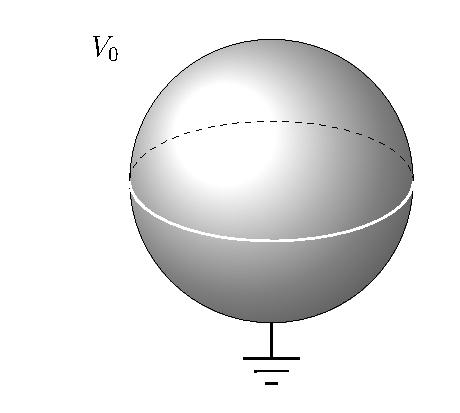
\includegraphics[scale=1]{Imagenes/esfera_5.eps}
    \caption{Configuración de la esfera para el ejercicio.}
\end{figure}
%Ref. Sepulveda (2004) Cap. 8 Funciones Especiales
\item Demuestra que la condición de completes de la base $\left\{ P_{n} (x) \right\}$ tiene la forma:
\begin{align*}
\delta (x - \pderivada{x}) = \dfrac{1}{2} \nsum_{n=0}^{\infty} \, P_{n} (x) \, P_{n} (\pderivada{x}) \hspace{1cm} n = 0, 1, 2, \ldots 
\end{align*}
%Ref. Arfken (2006) 12.5.4)
\item Demuestra que:
\begin{align*}
P_{n}^{n} (\cos \theta) = (2 \, n - 1)!! \, \sin^{n} \theta, \hspace{1.5cm} n = 0, 1, 2, \ldots
\end{align*}
%Ref.
\item Demuestra que evaluando el $P_{n}^{m}(0)$, se obtiene:
\begin{align*}
P_{n}^{m} (0) = \begin{cases}
(-1)^{\frac{(n-m)}{2}} \, \dfrac{(n + m)!}{2^{n} \bigg[ \left( \dfrac{n - m}{2} \right)! \left( \dfrac{n + m}{2} \right)! \bigg]}, & n + m \mbox{ par} \\
0, & n + m \mbox{ impar}
\end{cases}
\end{align*}
Demuestra adicionalmente que con $n + m$ par, el valor de $P_{n}^{m}(0)$ también se expresa como:
\begin{align*}
P_{n}^{m}(0) = (-1)^{\frac{(n-m)}{2}} \, \dfrac{(n + m - 1)!!}{(n - m)!!}
\end{align*}
%Ref. Arfken (2006) 12.7.1
\item Utilizando las formas conocidas de $L_{+}$ y $L_{-}$, demuestra que:
\begin{align*}
\scaleint{6ex} \big[ Y_{lm} \big]^{*} \, L_{-} \, \big( L_{+} \, Y_{lm} \big) \dd{\Omega} = \scaleint{6ex} \big( L_{+} \, Y_{lm} \big)^{*} \, \big( L_{+} \, Y_{lm} \big) \dd{\Omega}
\end{align*}
%Ref. Arfken (2006) 12.7.5
\item Verifica mediante cálculo explícito que:
\begin{align*}
L_{+} \, Y_{1}^{0} (\theta, \varphi) = - \sqrt{\dfrac{3}{4 \pi}} \, \sin \theta \, e^{i \varphi} = \sqrt{2} \, Y_{1}^{1} (\theta, \varphi)
\end{align*}
Estos signos (fase de Condon-Shortley) son una consecuencia de los operadores sucesivos $L_{+}$ y $L_{-}$.
%Ref. Arfken (2006) 12.8.3
\item El potencial de un electrón en el punto $\vb{r}_{e}$ en el campo de $Z$ protones en puntos $\vb{r}_{p}$ es:
\begin{align*}
\Phi = - \dfrac{e^{2}}{4 \pi \varepsilon_{0}} \, \nsum_{p=1}^{Z} \dfrac{1}{\abs{\vb{r}_{e} - \vb{r}_{p}}}
\end{align*}
\begin{enumerate}[label=\roman*)]
\item Demuestra que esto se puede escribir de la forma:
\begin{align*}
\Phi = - \dfrac{e^{2}}{4 \pi \varepsilon_{0} \, r_{e}} \, \nsum_{p=1}^{Z} \nsum_{\ell, m} \bigg( \dfrac{r_{p}}{r_{e}} \bigg)^{\ell} \dfrac{4 \pi}{2 \ell + 1} \big[ Y_{\ell}^{m} (\theta_{p}, \phi_{p}) \big]^{*} \, Y_{\ell}^{m} (\theta_{e}, \phi_{e})
\end{align*}
donde $r_{e} > r_{p}$.
\item ¿Cómo debe de escribirse $\Phi$ para $r_{e} < r_{p}$?
\end{enumerate}

\end{enumerate}

\end{document}